% Para documento texto corto
\documentclass[paper=letter,oneside,fontsize=12pt, parskip=full]{article}
%\documentclass[paper=letter,oneside,fontsize=11pt, parskip=full]{scrartcl}
%\documentclass{amsart}
%\documentclass[paper=letter,oneside,fontsize=12pt]{scrartcl}

% Establece dimensiones de los margenes
% \usepackage[inner=1.5cm,outer=3cm,top=2cm,bottom=4cm,
% bindingoffset=5mm]{geometry}
\usepackage[left=2cm,right=2cm,top=3cm,bottom=2cm,
bindingoffset=0cm, footskip=0.5cm, headheight=2cm]{geometry}

% Permite ingresar caracteres acentuados y especiales 
% sin necesidad de emplear comando
% utf8 codificacion de entrada Unicode (mas simbolos que ASCII)
\usepackage[utf8]{inputenc}

% Para usar graficos en archivos externos
\usepackage{graphicx}

% Tabla de tres secciones
\usepackage[flushleft]{threeparttable}

% T1 encoding for European, English, American text
\usepackage[T1]{fontenc}
% Fuente escalable
\usepackage{lmodern}

% Para definir colores
\usepackage{xcolor}
\usepackage{colortbl}


% Definicion de colores tabla cronograma
\definecolor{colorfa}{rgb}{0.3569,0.608,0.8353}
\definecolor{colorfb}{rgb}{0.4392,0.678,0.2784}
\definecolor{colorfc}{rgb}{1.0000,0.361,0.0000}
\definecolor{colorsem}{rgb}{0.1804,0.455,0.7098}
\definecolor{colorfd}{rgb}{0.9294,0.490,0.1922}
\definecolor{colorfe}{rgb}{0.2667,0.329,0.4157}

% Definicion comandos tabla cronograma
\newcommand{\fa}{\cellcolor{colorfa}}
\newcommand{\fb}{\cellcolor{colorfb}}
\newcommand{\fc}{\cellcolor{colorfc}}
\newcommand{\sem}{\cellcolor{colorsem}}
\newcommand{\fd}{\cellcolor{colorfd}}
\newcommand{\fe}{\cellcolor{colorfe}}

\begin{document}
	
	\section{Propuesta de cambios en TEG}
	
	\subsection{Cambios en diseño del dispositivo Cendit11713}
	
		\begin{center}
			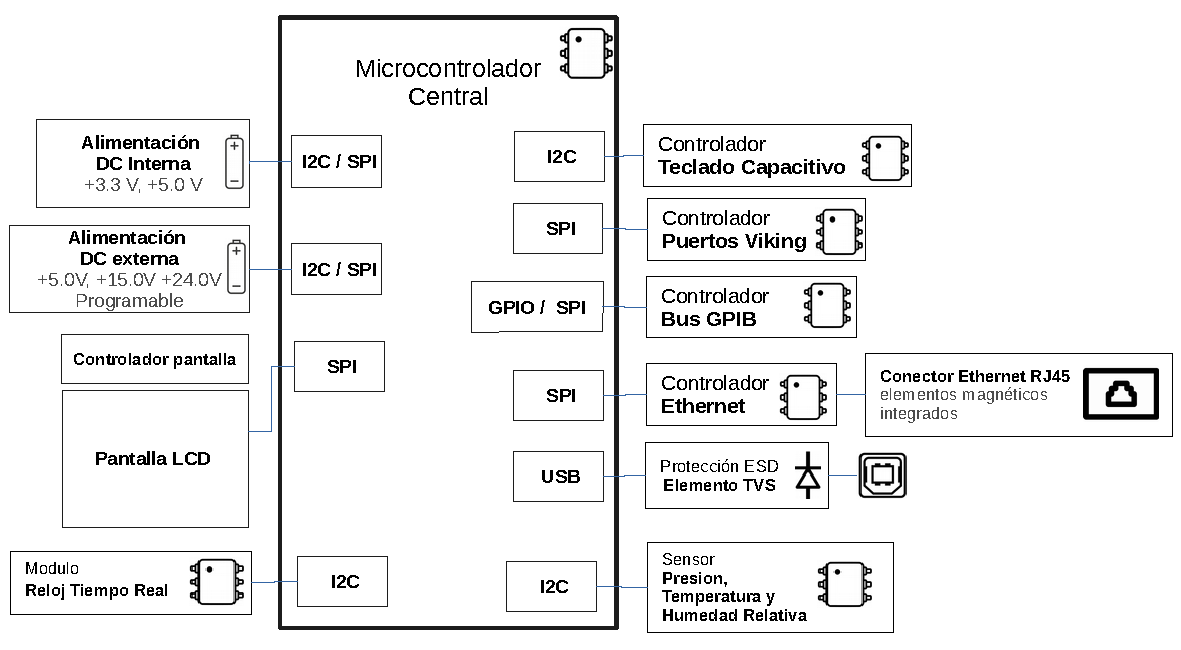
\includegraphics[width=16cm]{Cendit11713BloquesAntes.pdf} \\
		\end{center}

		\begin{center}
			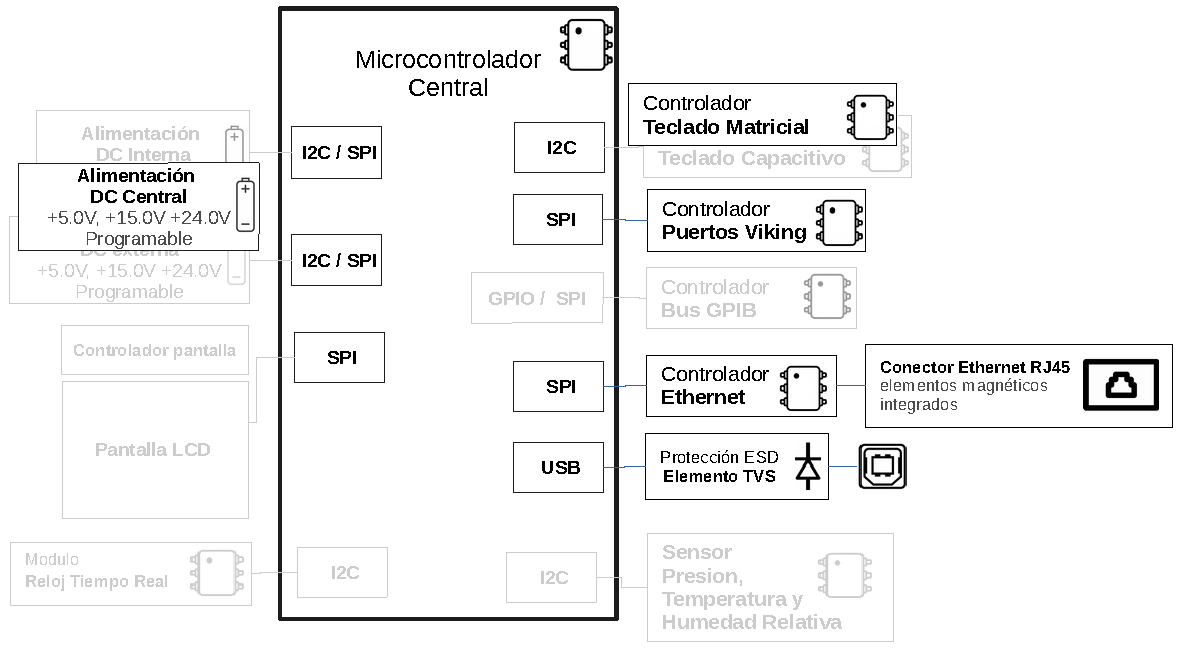
\includegraphics[width=16cm]{Cendit11713BloquesDespues.pdf}
		\end{center}	
	
	\subsection{Pautas}
	
	\begin{enumerate}
	
		\item Una solución de tipo “quick and dirty” para el dispositivo electrónico. Esta es la solución para la UCV. Se realizará una tarjeta madre PCB los más simple posible, tal vez empleando un integrado de tipo thru-hole (no de montaje superficial) en donde reside el micro central acompañado de varios conectores (tiras de pines – pin headers) en cada uno de sus puertos. En estas tiras de pines por medio de cable de cinta se conectará en uno un teclado matricial simple (de 4 x 4), en los otros se conectan las tarjetas expansoras, una de ellas con los transceptores para el bus GPIB.
		
		\item Una aplicación del mismo tipo, “quick and dirty”, únicamente con cuatro pantallas para cada proceso de medición, configuración y calibración para: medición de figura de ruido, medición de potencia de ruido, medición de ganancia, configuración. Esta aplicación es para la UCV. En principio no posee capacidad para corrección por medio de parámetros S de los dispositivos de conexión ni capacidad de simulación. Estas características se agregaran si hay tiempo y una vez completada las tarjetas PCB.
		
		\item Me preocupa el desarrollo del bus GPIB, en cuanto no he podido conseguir los IC transceivers de bus. Además, la documentación que he conseguido en superficial, a nivel de usuario, no detalla la capa de comunicaciones (señales + diagramas de tiempo.). La especificación de este bus IEEE-488 no se consigue de forma libre, hay que pagar por ella. En cambio, para el controlador LAN, en la página de Microchip abunda la información.
	
	\end{enumerate}
	
	\subsection{Cronograma inicial TEG}
	
		\begin{threeparttable}[!h]
			\centering
			\arrayrulecolor{gray}
			\setlength{\extrarowheight}{4pt}		
			\resizebox{\textwidth}{!}{
				\begin{tabular}{|c|l|l|l|l|l|l|l|l|l|l|l|l|l|l|l|l|l|l|l|l|l|l|l|l|l|l|l|l|}
					\hline 			
					\textbf{Semanas} & 1 & 2 & 3 & 4 & 5 & 6 & 7 & 8 & 9 & 10 & 11 & 12 & 13 & 14 & 15 & 16 & 17 & 18 & 19 & 20 & 21 & 22 & 23 & 24 & 25 & 26 & 27 & 28 \\
					\hline
					\textbf{Fase 1}
					& \fa & \fa & \fa & \fa & \fa & \fa & & & & & & & & & & & & & & & & & & & & & & \\			
					\hline			
					\textbf{Fase 2} & & & & & & & \fb & \fb & \fb & \fb & \fb & \fb & \fb & \fb & \fb & \fb & \fb & & & & & & & & & & & \\
					\hline
					\textbf{Fase 3} & & & & & & & & & & & & & & & & & & \fc & \fc & \fc & \fc & \fc & & & & & & \\	
					\hline		
					\textbf{Seminario} & & & & & & & & & & & & & & \sem & & & & & & & & & & & & & & \\
					\hline
					\textbf{Fase 4} & & & & & & & & & & & & & & & & & & & & & & & \fd & \fd & \fd & \fd &  & \\
					\hline
					\textbf{Fase 5} & & & & & & & & & & & & & & & & & & & & & & & & & & & \fe & \fe \\
					\hline	
				\end{tabular}
			}
			\begin{tablenotes}
				\item {\tiny Fecha de inicio: 6 de Marzo de 2017.} 
				\item {\tiny Jornada de 8 horas diarias, lunes a viernes, de 8:00 AM a 12:00 M y de 1:30 PM a 4:30 PM.}
			\end{tablenotes}
		\end{threeparttable}
	
	\subsection{Contabilidad horaria}
	
		\begin{figure}[h!]
			\centering
			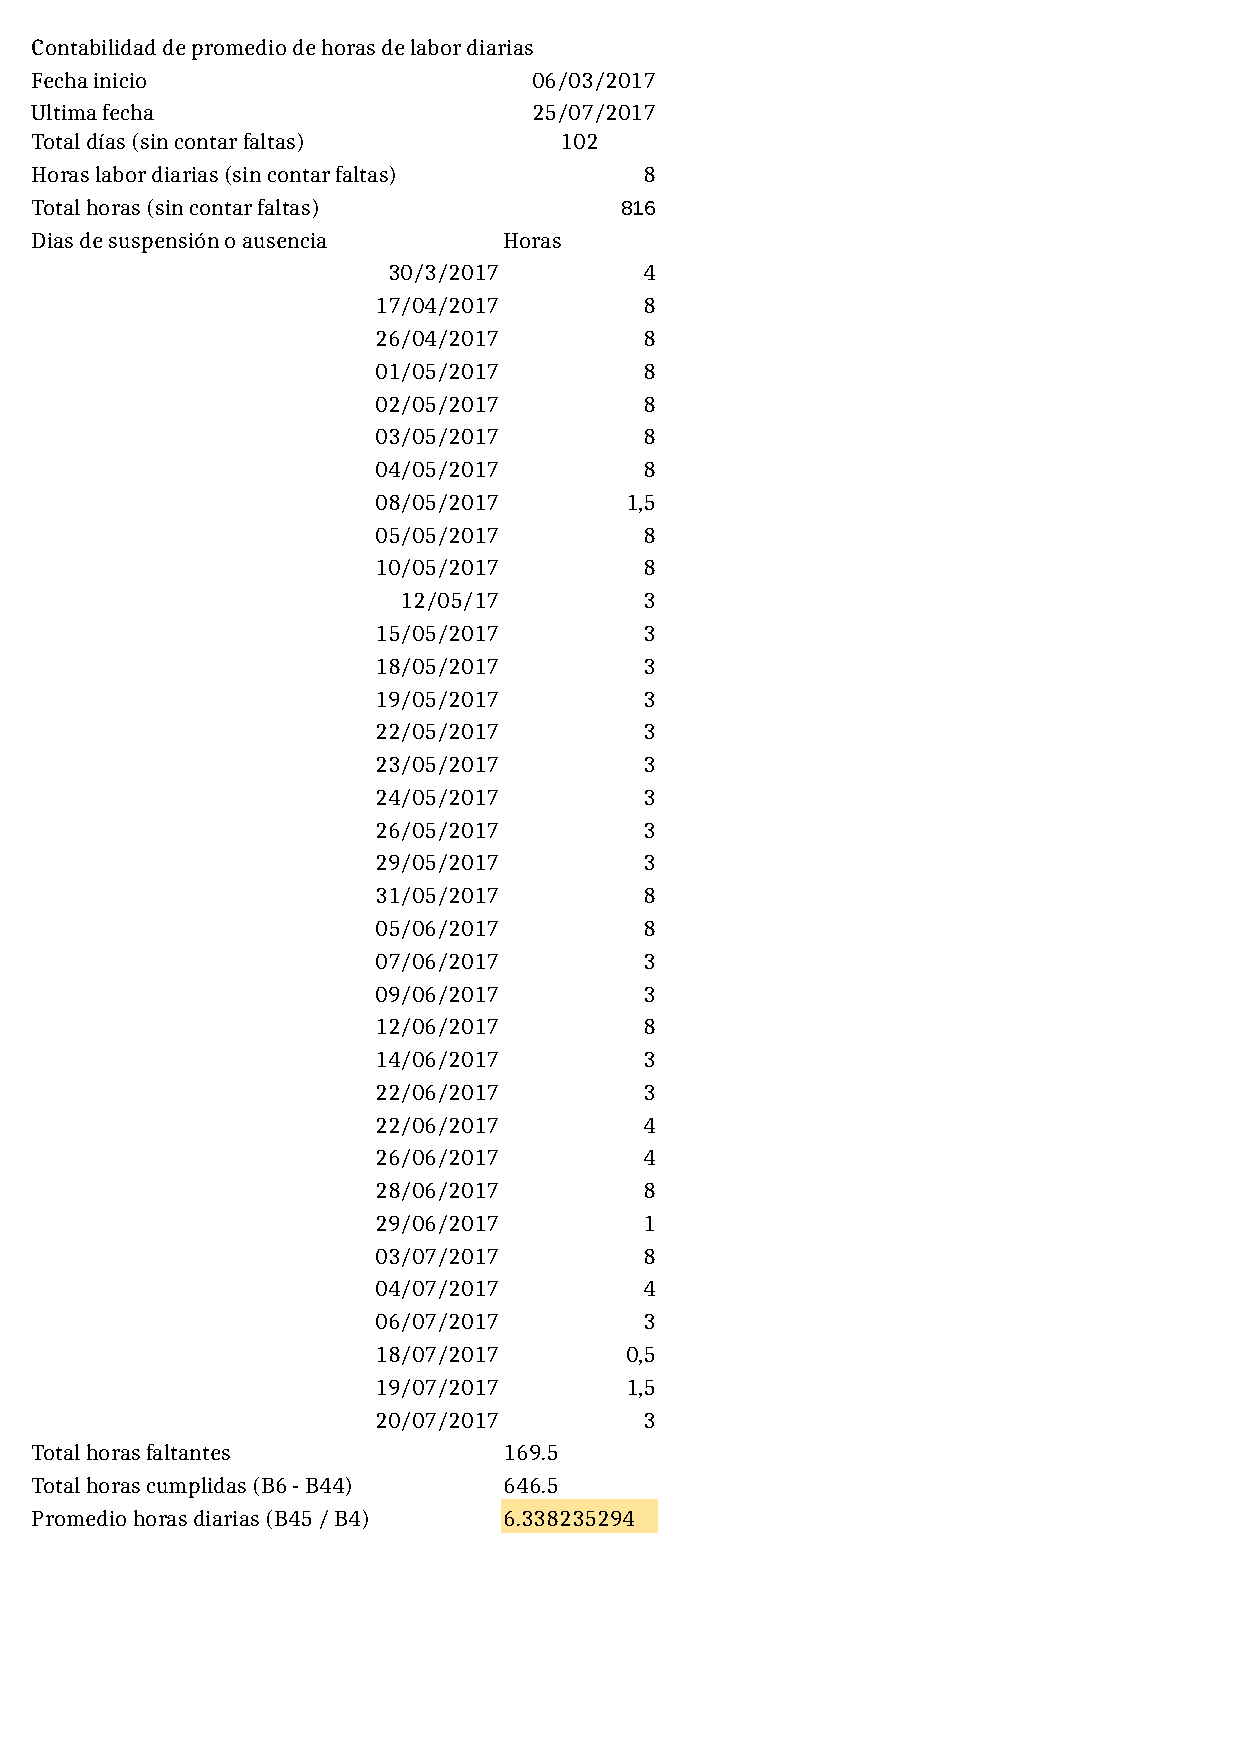
\includegraphics[width=10cm]{ContabilidadHorasPasantia.pdf}
		\end{figure}
	
\end{document}